\chapter{FORMAL ANALYSIS}
\label{ch:formalAnalysis}%
% The \label{...}% enables to remove the small indentation that is generated, always leave the % symbol.
In this chapter alloy analysis will be used in order to demonstrate the validity of the model, pointing out some peculiarities hard to notice given the previous UML representation.
\section{Alloy Code}
\label{sec:alloyCode}
\begin{lstlisting}[language=alloy]
sig PaymentApi {}

sig Time {timeStamp : one  Int} {timeStamp >= 1}

abstract sig EnergyProvider{}

sig DSO extends EnergyProvider{}

------------------- DRIVER 
sig Driver {
    drives: one ElectricVehicle,
    calendar: set CalendarEvent, 
    uses: some eMSP,
    driverPayment: uses -> one PaymentApi,
    receives: set Suggestion,
    books: set Booking
}

sig Booking {
    station: one ChargingStation,
    socket: one ChargingSocket,
    time: one Time,
}{one this.~creates and one this.~books and socket in station.sockets}

sig ElectricVehicle {
    routes: set NavigationRoute
} { one this.~drives}

sig NavigationRoute {} { one this.~routes}

sig CalendarEvent {}{one this.~calendar}

------------------- CPO 
sig CPO {
    utilizes: one CPMS,
    cpoPayment: eMSP -> lone PaymentApi
}

sig CPMS {
    manages: some ChargingStation,
    creates: set Booking,
    associates: set eMSP
}{one this.~utilizes}

sig ChargingStation {
    sockets: some ChargingSocket,
    price: ChargingType -> lone Price,
    energyProvider: some EnergyProvider
}{one this.~manages}

sig Battery extends EnergyProvider{}{one this.~energyProvider}

sig Price {} 

sig ChargingSocket {
    type: one ChargingType
} {one this.~sockets}
// represents a charging type, such as slow, fast, rapid...
sig ChargingType {}

------------------- eMSP 
sig eMSP {
    supports: some PaymentApi,
    generates: set Suggestion,
    map: one Map,
}
sig Map {
    contains: set ChargingStation
}{one this.~map}

sig Suggestion {
    event: set CalendarEvent,
    navigation: set NavigationRoute,
    vehicle: one ElectricVehicle,
    suggestedStation: one ChargingStation
}{one this.~generates and one this.~receives}

------------------- FACTS
// for each driver and eMSP there is only one payment method used for that eMSP and that payment method is supported
fact driverUsesOnlySupportedPayments{
    all d:Driver, e:eMSP | e in d.uses implies (one p:PaymentApi | 
        p = e.(d.driverPayment)) and (e.(d.driverPayment) in e.supports)
}

//  for each CPO and eMSP there is only one payment method used for that eMSP and that payment method is supported
fact CPOUsesOnlySupportedPayments{	
    all c:CPO, e:eMSP | (e in c.utilizes.associates iff (one p:PaymentApi | 
    p = e.(c.cpoPayment))) and (e.(c.cpoPayment) in e.supports)
}

// suggestions are only based on data from the driver receiving that suggestion
fact useOnlyDataFromReceivingDriver{
    all s:Suggestion | (
	(all c:CalendarEvent | c in s.event iff c.~calendar = s.~receives) and
	(all n:NavigationRoute | n in s.navigation iff
        n.~routes.~drives=s.~receives) and
	(all v:ElectricVehicle | v = s.vehicle iff v.~drives= s.~receives)
	)
}

// an eMSP can suggest only a charging station present in its map
fact onlySuggestStationInMap{
    all s:Suggestion | s.suggestedStation in s.~generates.map.contains
}

// an eMSP can send suggestions only to drivers using that eMSP
fact onlySuggestionsForAssociatedDrivers{
    all s:Suggestion | s.~generates in s.~receives.uses
}

// if a price exists then it's associated to some charging station
fact everyPriceConnected{
    no p:Price | p not in ChargingType.(ChargingStation.price)
}

// if a charging type is supported by some charging station then there exists a single price set by that charging station for that charging type
fact ChargingTypeMatchesSocketType {
    all s:ChargingStation, t:ChargingType | (t in s.sockets.type iff (one           p:Price | p = t.(s.price)))
}

// a Driver can do a booking only for a charging station in a map of one of his used eMSPs, associated with the CPMS of said station
fact onlyeMSPAssociatedBookings{
    all b:Booking, d:Driver | b in d.books implies 
        (some e: eMSP | e in ((b.station).~contains).~map and e in d.uses and e in (b.~creates).associates)
}

// every booking made on the same socket must be on different times
fact DifferentBookingsDifferentTimes{
	all disj b1, b2: Booking | b1.socket = b2.socket implies b1.time != b2.time
}

// every charging station appears in a map iff the CPMS managing that charging station is associated to that map's eMSP
fact ChargingStationsInEmspMap {
    all s: ChargingStation, m: Map | s in m.contains iff (m.~map in                 (s.~manages).associates)
}

------------------- ASSERTIONS
assert NoUnmatchedSocketAndCharging {
    no c:ChargingStation | some t: ChargingType | (t in c.sockets.type and no       p:Price | p in t.(c.price)) or (t in (c.price).Price and 
        no s: ChargingSocket | s in c.sockets and s.type = t)
}
--check NoUnmatchedSocketAndCharging

assert NoDriverWithUnsupportedPayment {
    no d: Driver | (some e: eMSP | e in d.uses and (no p: PaymentApi | p in e.      (d.driverPayment) and p in e.supports) or 
        (e.(d.driverPayment) not in e.supports))
}
--check NoDriverWithUnsupportedPayment

assert NoCPOWithUnsupportedPayment {
    no c:CPO | some e:eMSP | e in c.utilizes.associates and (no p: PaymentApi |     p in e.(c.cpoPayment) and p in e.supports)
        or (e.(c.cpoPayment) not in e.supports)
}
--check NoCPOWithUnsupportedPayment

assert NoBookingWithoutAssociationOrUsage{
    no b: Booking | no e:eMSP | (e in ((b.station).~contains).~map and e in         (b.~creates).associates) or e not in (b.~books).uses
}
--check NoBookingWithoutAssociationOrUsage

assert NoBookingsAtSameTime {
	no disj b1, b2: Booking | b1.socket = b2.socket and b1.time = b2.time
}
--check NoBookingsAtSameTime

assert NoSuggestionWithNotAssociatedChargingStations {
    no s: Suggestion|  s.~generates not in (s.suggestedStation).~manages.associates
}
--check NoSuggestionWithNotAssociatedChargingStations

------------------- DYNAMIC MODELLING
// add a booking
pred addBooking[d:Driver, d':Driver, b:Booking]{
    d'.drives = d.drives
    d'.calendar = d.calendar
    d'.uses =  d.uses
    d'.driverPayment = d.driverPayment
    d'.receives = d.receives
    d'.books = d.books + b
}
-- run addBooking for 5

// receive a suggestion
pred receiveSuggestion[d:Driver, d':Driver, s:Suggestion]{
    d'.drives = d.drives
    d'.calendar = d.calendar
    d'.uses =  d.uses
    d'.driverPayment = d.driverPayment
    d'.receives = d.receives + s
    d'.books = d.books
} 

-- run receiveSuggestion for 5

// add a charging station
pred addChargingStation[c:CPMS, c':CPMS, s:ChargingStation]{
    c'.manages = c.manages + s
    c'.creates = c.creates
    c'.associates = c.associates
}
-- run addChargingStation for 5
// associate CPMS to new eMSP
pred associateToEeMSP[c, c':CPMS, e:eMSP]{
    c'.associates = c.associates + e
    c'.manages = c.manages
    c'.creates = c.creates
}
-- run associateToEeMSP for 5

------------------- STATIC MODELLING
pred world1 {
    # ChargingStation = 3
    # ChargingSocket = 4
    # Driver = 3
    # Price = 3
    # uses  = 4
    # ChargingType = 3
    # PaymentApi = 3
    # associates = 3
    # eMSP = 3
    # CPO = 2
    # CPMS = 2
    # DSO = 2
    # Battery = 1
    # Booking = 0
    # NavigationRoute = 0
    # Suggestion = 0
    # CalendarEvent = 0
    # Time = 0
}
-- run world1 for 5
pred world2 {
    # ChargingStation = 3
    # ChargingSocket = 4
    # Driver = 2
    # Price = 2
    # uses  = 2
    # ChargingType = 3
    # PaymentApi = 1
    # associates = 2
    # eMSP = 1
    # CPO = 2
    # CPMS = 2
    # DSO = 1
    # Booking = 2
    # Battery = 0
    # NavigationRoute = 2
    # Suggestion = 2
    # CalendarEvent = 2
    # Time = 2
}

run world2 for 5
\end{lstlisting}
\newpage
\subsection{Results}
\label{subsec:results}
No assertion gives a counterexample instance, hence the model should be well-posed.
\begin{figure}[H]
    \begin{center}
    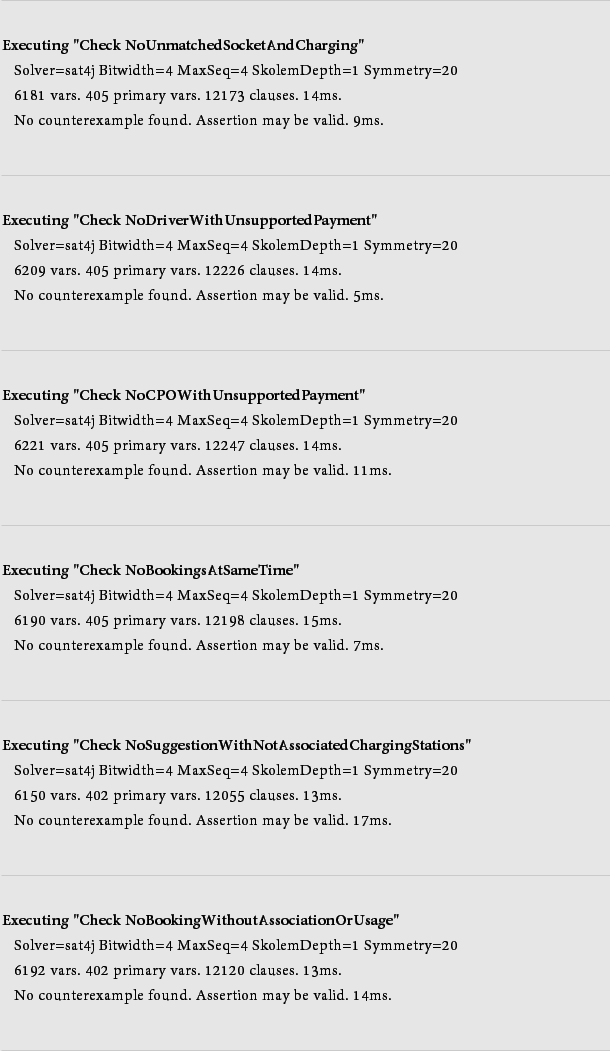
\includegraphics[
        width=\textwidth,
        height=0.35\textheight,
        keepaspectratio]{Alloy/Assert}
    \caption{Assertions Results}
    \label{fig:AssertionsResults}
    \end{center}
\end{figure}
\section{Models}
\label{sec:models}
\subsection{First Model}
\label{subsec:firstModel}
In figure \ref{fig:World_1} the most important relations of the model are represented. In particular, it's possible to notice that the map of an eMSP shows only the charging stations managed by a CPMS associated with that eMSP. \\
Another interesting relation shows that both Drivers and CPOs have to use a payment method (PaymentAPI) supported by the eMSP to which they are directly (for Drivers) or indirectly (for CPOs, through their CPMS) linked.
\subsection{Second Model}
\label{subsec:secondModel}
In figure \ref{fig:World_2} it is possible to see how the bookings and suggestions work. In particular, Drivers can create a booking, through a used eMSP, on a station's socket only if that station is managed by a CPMS associated with said eMSP. Also, the suggestions can be received by Drivers based on their vehicle, navigation routes and calendar events. Similarly to Bookings, they can be suggested a charging station only if the eMSP that generates the suggestion is associated with the CPMS that manages said station.
\begin{figure}[H]
    \begin{center}
    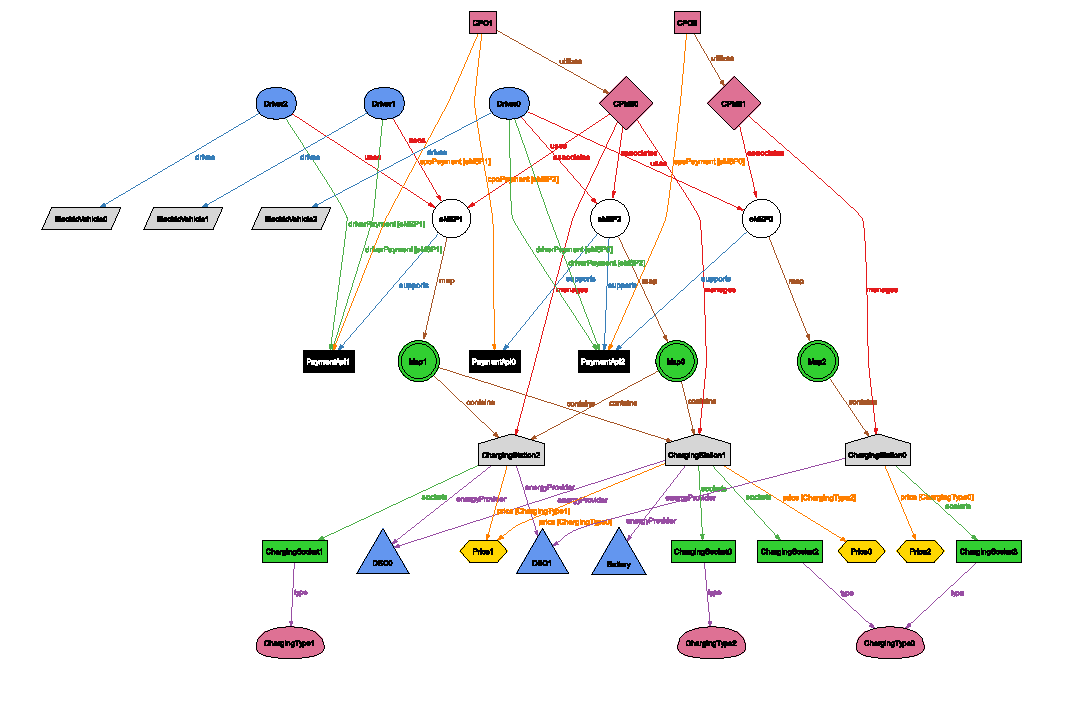
\includegraphics[
        width=\textwidth,
        height=\textheight,
        keepaspectratio]{Alloy/World_1}
    \caption{World 1}
    \label{fig:World_1}
    \end{center}
\end{figure}
\begin{figure}[H]
    \begin{center}
    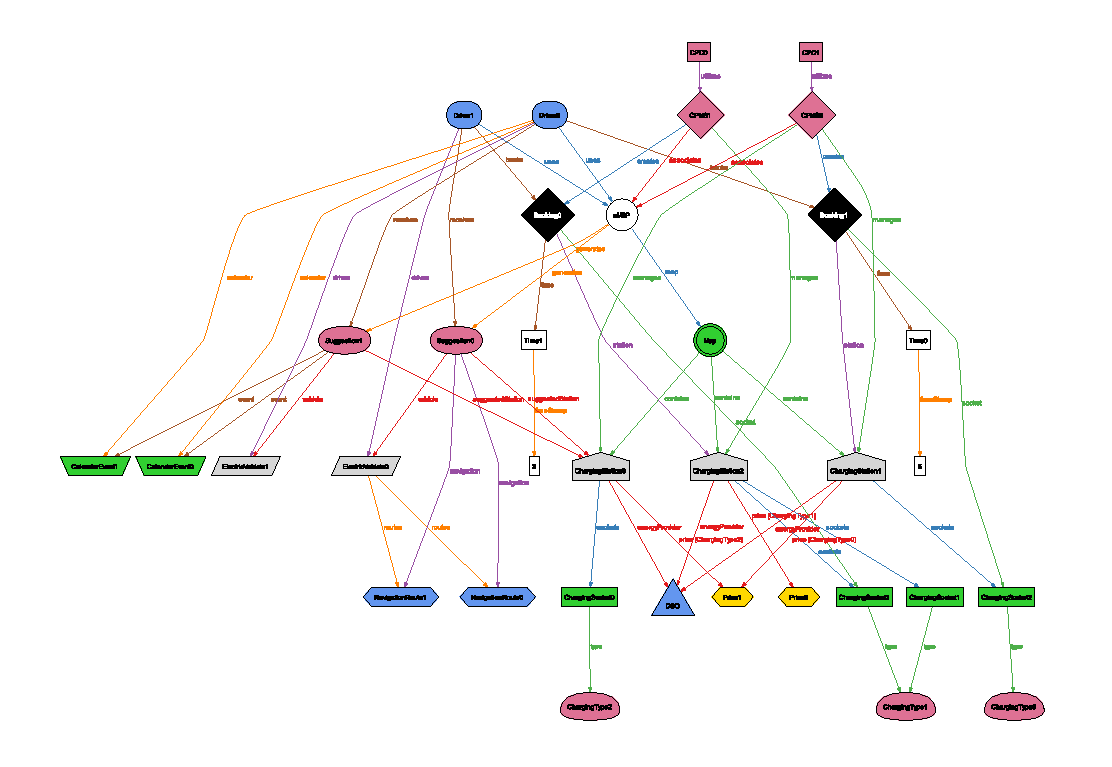
\includegraphics[
        width=\textwidth,
        height=\textheight,
        keepaspectratio]{Alloy/World_2}
    \caption{World 2}
    \label{fig:World_2}
    \end{center}
\end{figure}
\subsection{Dynamic Model}
Here below there is an example instance found running the \textit{addBooking} predicate
\label{subsec:dynamicModel}
\begin{figure}[H]
    \begin{center}
    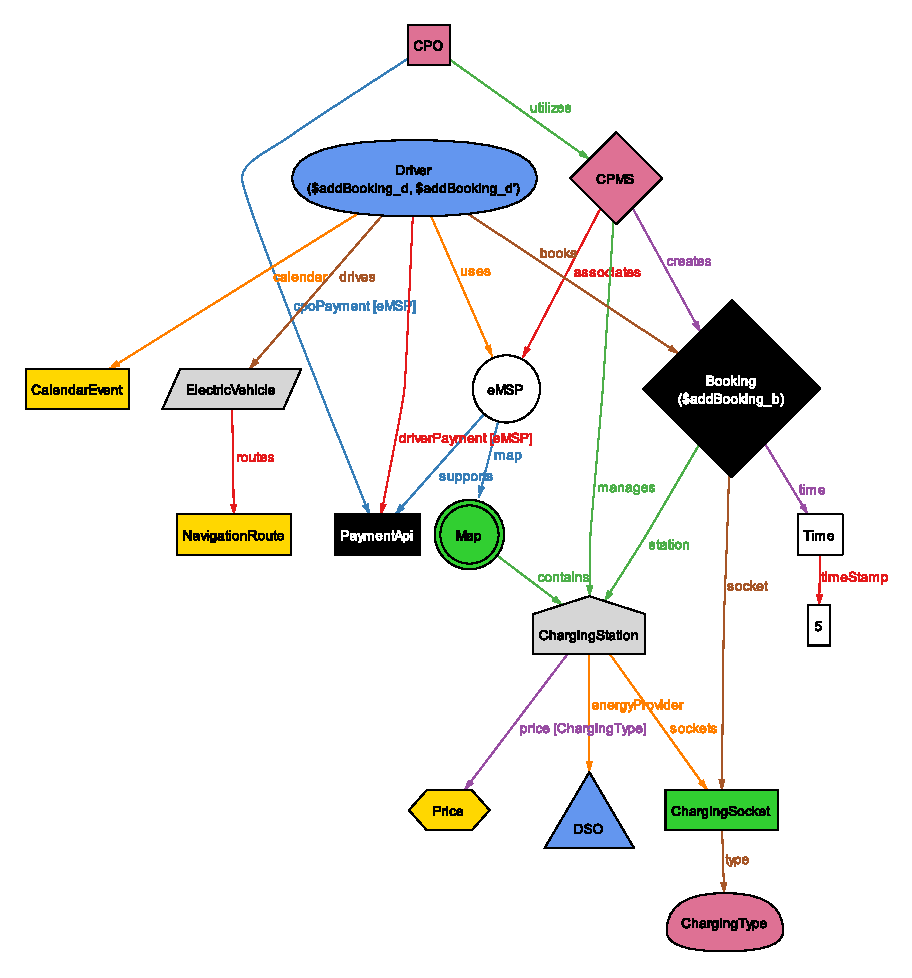
\includegraphics[
        width=\textwidth,
        height=0.5\textheight,
        keepaspectratio]{Alloy/AlloyBooking}
    \caption{Booking Example}
    \label{fig:bookingExample}
    \end{center}
\end{figure}